\documentclass[tikz,border=2pt]{standalone}
\usepackage{tikz}
\usetikzlibrary{positioning}
\begin{document}
	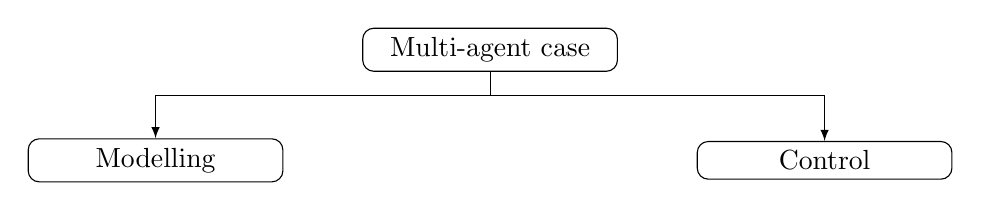
\begin{tikzpicture}[
	main/.style={rectangle, rounded corners, text centered, text width=3cm, draw=black},
	aux/.style={}
	]	
	
		\node (multiagent) [main] {Multi-agent case};
				\node (aux10) [aux, below=of multiagent] {};	
				\node (multiagentcontrol) [main, right=2.5cm of aux10] {Control};
				\node (multiagentmodelling) [main, left=2.5cm of aux10] {Modelling};

	\draw [-latex] (multiagent.south)--++(0,-.3)-| (multiagentcontrol.north);
	\draw [-latex] (multiagent.south)--++(0,-.3)-| (multiagentmodelling.north);
	

	
	\end{tikzpicture}
\end{document}